\section{A model-checker for process models\label{section:tool-model-checker}}

Our model-checker for guarded hMSC extends the compositional model-checking technique presented in \cite{Giannakopoulou:2003}. The latter allows model-checking LTS state machines against FLTL safety properties. Our tools extends this to the model-checking of g-hMSC and g-LTS. 

The model-checking technique is illustrated on Fig.~\ref{image:model-checking-technique}. Let us read it backwards:
\begin{itemize}
\item Roughly, compositional model-checking consists in searching for an accepting state in the composition of two automata: one for the model being checked (top), the other for the negation of the checked property (the tester automaton at bottom). Note that our tool is limited to safety properties, for which such tester always exists (see Section \ref{subsection:background-property-and-tester-automata}).
\item The model automaton is synthesized from the g-hMSC and fluent definitions using the techniques described in Chapter \ref{chapter:deductive}. At first glance (see below), it is the pure LTS capturing the trace semantics of the input g-hMSC.
\item The tester automaton is synthesized using the technique described in \cite{Giannakopoulou:2003}. Roughly, it consists in translating the negation of the checked safety property to a B\"uchi automaton \cite{Giannakopoulou:2002}; the latter is then composed with fluent automata and with a synchronizer automaton forcing the transition on the B\"uchi automaton after every system event. 
\end{itemize} 

\begin{figure}
\centering\scalebox{.525}{
  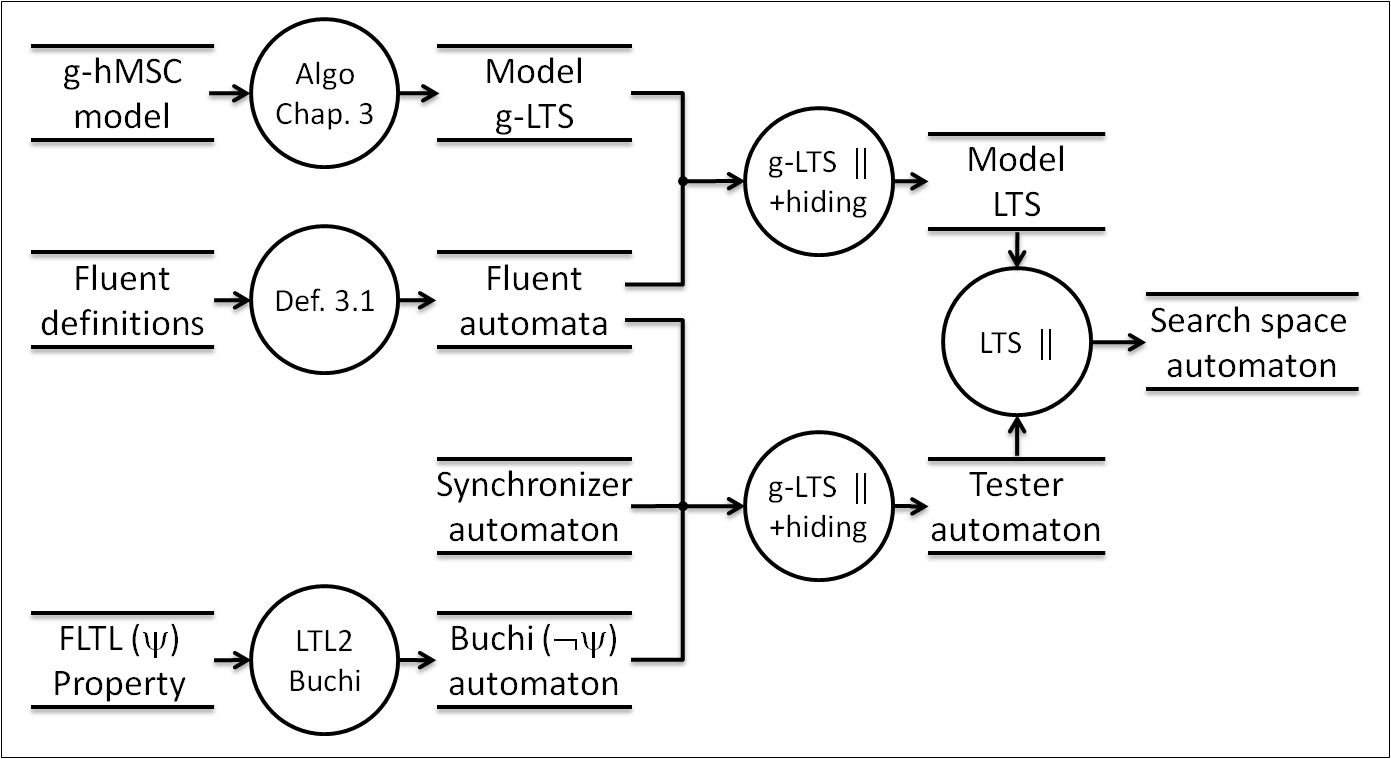
\includegraphics[trim=3mm 3mm 3mm 3mm, clip]{src/7-tool-support/images/model-checking-technique}}
  \caption{Model-checking guarded hMSC: automaton compositions\label{image:model-checking-technique}}
\end{figure}

The main differences between our model-checker and the technique described in \cite{Giannakopoulou:2003} and its implementation in LTSA are the following.
\begin{itemize}

\item Unlike LTSA, our tool makes use of guarded automata instead of simple LTS. Guarded automata are a flavor of guarded LTS that distinguishes between accepting and non-accepting states. 

Guarded automata allows us to capture B\"uchi automata, fluent automata, LTS, g-LTS and standard automata with only one data structure. Only one composition algorithm is also required for apparently different compositions operators in Fig.~\ref{image:model-checking-technique}. 

The composition operator on guarded automata extends the one described in Section \ref{subsection:glts-operators} by making a distinction between accepting and non-accepting states. This operator reduces to g-LTS composition when composed automata have all accepting states; it reduces to LTS composition if they don't have guards either. 

Last, this operator requires computing the conjunctions of guards and checking their satisfiability. Our tool uses Binary Decision Diagrams (BDD) to implement this efficiently \cite{Bryant:1986}. 

\item LTSA checks temporal properties for a specific initial state, specified through an initial value for each fluent. Guarded models use an initial condition $C_0$ instead (see Sections~\ref{section:background-process-models} and \ref{section:deductive-glts}). Such condition actually captures a class of fluent initial states. 

Therefore, our tool must check the temporal property for any initial state satisfying the initial condition. This simply requires the definition of fluent automata given in Section~\ref{subsection:from-glts-to-lts} instead of the one given in \cite{Giannakopoulou:2003}; the synchronizer automaton must also be slightly adapted so as to first synchronize with guarded transitions from initial states of the fluent automata.

\item For effective feedback in case of a property violation our tool needs to keep track of the initial fluent assignment during search. To achieve this, the model and tester automata are not pure LTS; instead, they have fluent value assignments on all transitions from their initial state. These transitions capture the choice of an fluent initial state at the beginning of every trace. 

To achieve this, the construction of the model and tester automata is slightly changed. First, observe that their construction relies on a composition with fluent automata. In both cases, this composition yields guarded transitions from the initial state. By construction, these guards reduce to simple conjunctions of fluent literals, that is, a form of fluent value assignments. The last step of the construction of these automata usually consists in hiding guards. In our case, this hiding step is simply updated in such a way that these guarded transitions from the initial state are kept. All other guards are still hidden. 

\end{itemize}

\subsubsection*{Discussion}

The tool is implemented in Java 1.5.0 and has been tested on a few case studies (see, e.g. \cite{Damas:2010}). Numerous improvements could be made:
\begin{itemize}
\item Our model-checking procedure relies on three costly compositions: one for building the model, one for the tester and one for the model-checking itself. 

The third one is implemented as an effective search: it ends and returns a trace as soon as a violation is found, that is, without explicitely representing the composed automaton. In contrast, our tool explicitely represents the tester and the model automata. 

There are both advantages and inconvenients in doing so. Verifying a property requires explicitely representing the whole state space of the guarded hMSC, which has been shown exponential in the number of fluents. An implicit search strategy could be implemented here. However it would prove less efficient for verifying more than one safety property on the same model. Indeed, the model automata can be minimized if explicitly captured. A search strategy would not profit from this state space reduction.

\item Unlike LTSA, our tool does not support model-checking of liveness properties. The procedure described in \cite{Giannakopoulou:2003} could certainly be adapted to guarded models in a similar way as for safety properties.
\end{itemize}

%The logical architecture of our model-checker is depicted in Fig.~\ref{image:model-checker}. Its implementation mostly relies on three main modules:

%\begin{figure}
%\centering\scalebox{.525}{
%  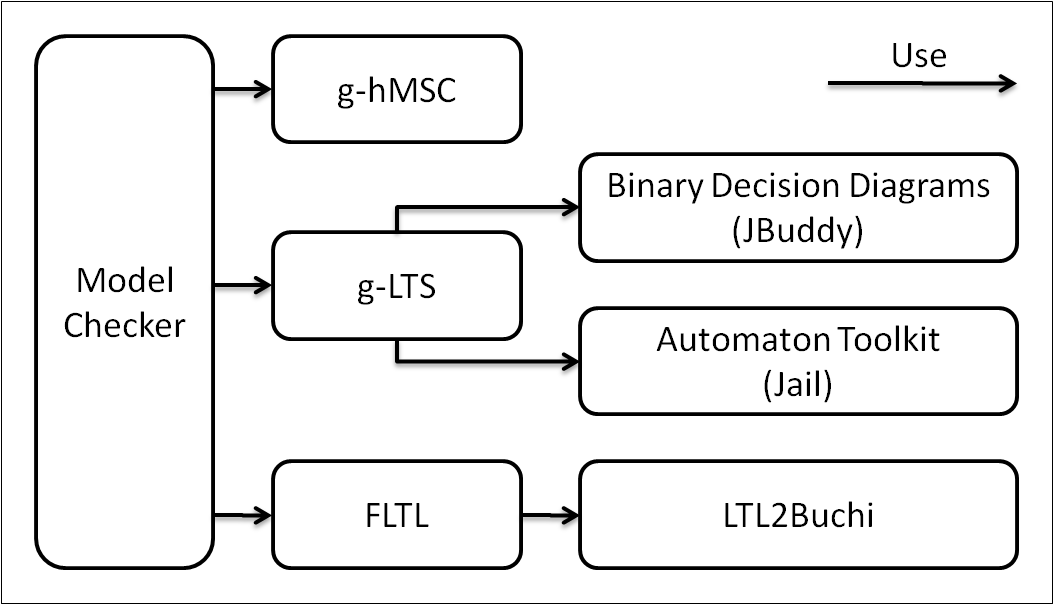
\includegraphics[trim=3mm 3mm 3mm 3mm, clip]{src/7-tool-support/images/model-checker-architecture}}
%  \caption{Architecture of the g-hMSC model checker\label{image:model-checker}}
%\end{figure}

%\begin{description}
%\item[Guarded automata] The first module is an implementation of guarded automata. This module reuses our abstract automaton toolkit, namely Jail (which stands for Java Automaton and Induction Library) and a library called JavaBDD\footnote{available at http://javabdd.sourceforge.net/ (last retrieved 2011-08-25)} for efficiently manipulating guards through Binary Decision Diagrams (BDD) \cite{Bryant:1986}.

%Jail implements an automaton data structure together with standard algorithms:  minimization, determinization, composition, etc. It has been designed as a fairly abstract library in that it allows states and edges of automata to be decorated with any \emph{(key,value)} pairs. Jail algorithms can be configured to perform specific operations on such decorations when manipulating states and edges. As standard automaton algorithms often compute and/or merge sets of states and edges, Jail provides built-in implementations of aggregation operators (sum, avg, min, max, set union, set intersection, and so on).

%A specific configuration of the composition algorithm template in Jail yields the composition operator used on guarded automata. In particular, an aggregation operator for edges relies on BDDs for implementing the conjunction of guards.

%\item[FLTL] This second module implements fluents and FLTL temporal properties with the use of the LTL2Buchi\footnote{available at http://ti.arc.nasa.gov/profile/dimitra/projects-tools/ (last retrieved 2011-08-25)} library \cite{Giannakopoulou:2002}. 

%LTL2Buchi is used to parse LTL specifications and translates them to B\"uchi automata. Our FLTL module interfaces with LTL2Buchi and translates its B\"uchi automata in our g-LTS. It also translates fluent definitions to g-LTS as explained in Section~\ref{subsection:from-glts-to-lts}.

%\item[Guarded hMSC] This structural module implements Guarded hMSC. It mostly consists in the implementation of a graph made of tasks and decision nodes and an API to build them programmatically.
%\end{description}

%The main module of the model checker provides an API for deriving guarded LTS and LTS from guarded hMSC as well as model-checking them. 
